\documentclass{TDP005mall}
\usepackage{graphicx}
\usepackage{float}
\graphicspath{ {./images/} }


\newcommand{\version}{Version 1.0}
\author{
  Ismail Safwat, \url{saysa289@student.liu.se}}
\title{Kravspecifikation}
\date{2022-11-12}
\rhead{Ismail}



\begin{document}
\projectpage
\section{Revisionshistorik}
\begin{table}[!h]
\begin{tabularx}{\linewidth}{|l|X|l|}
\hline
Ver. & Revisionsbeskrivning & Datum \\\hline
1.0 & Kravspecifikation skapad & 2022-11-12 \\\hline
%1.1 & Kravspecifikation korrigerat enligt feedback & 2020-11-18 \\\hline
%1.2 & Kravspecifikation kompletterad & 2020-11-27 \\\hline
\end{tabularx}
\end{table}


\section{Spelidé}
 Spelet kommer utspela sig i en två-dimensionell värld med ett rakt kameraperspektiv. Fiender som har geometriska former kommer att komma närmare och närmare och det är spelarens uppgift att förstöra alla former innan det är för sent.
 
\section{Målgrupp}
 Spelet riktar sig till alla som är intresserade av arkadspel och passar alla åldersgrupper. 

\section{Spelupplevelse}
 Att skjuta på fienderna(former) och komma närmare till seger är stimulerande. Utmaningen är att förstöra fienderna innan de kolliderar med spelaren.

\section{Spelmekanik}
 Spelet kommer att ske i realtid. För att flytta eller röra på skytten ska spelaren använda tangentknapparna vänster (←) och höger (→). För att skjuta kommer space-knappen användas. Utanför spelet kommer space-knappen också att användas för att välja alternativ.

\section{Regler}

\subsection{Spelplan}
 Spelplanen har en fast och fixerad storlek och utseende. Spelaren och fienderna kommer förstås inte kunna röra sig bortom spelplanens kanter.

\subsection{Spelare}
 Spelaren styrs av användaren och kan bara röra sig åt vänster och höger. Spelaren och fiender kan kollidera med varandra men de kan aldrig gå igenom varandra. Om en kollision sker är spelet över.

\subsection{Fiender}
 Fienderna kommer att röra sig vänster/höger och när de kommer vid sidan av spelplanen kommer de att förflyttas ner. Om en fiende krockar med spelaren då slutar spelet. Om spelaren lyckas döda alla fiender har spelaren vunnit. Det kommer att finnas två olika typer av fiender det vill säga att de kommer ha olika former såsom triangel, fyrkant, rektangel, cirkel och så vidare.

\newpage

\section{Visualisering}

\begin{figure}[h!]
    \centering
    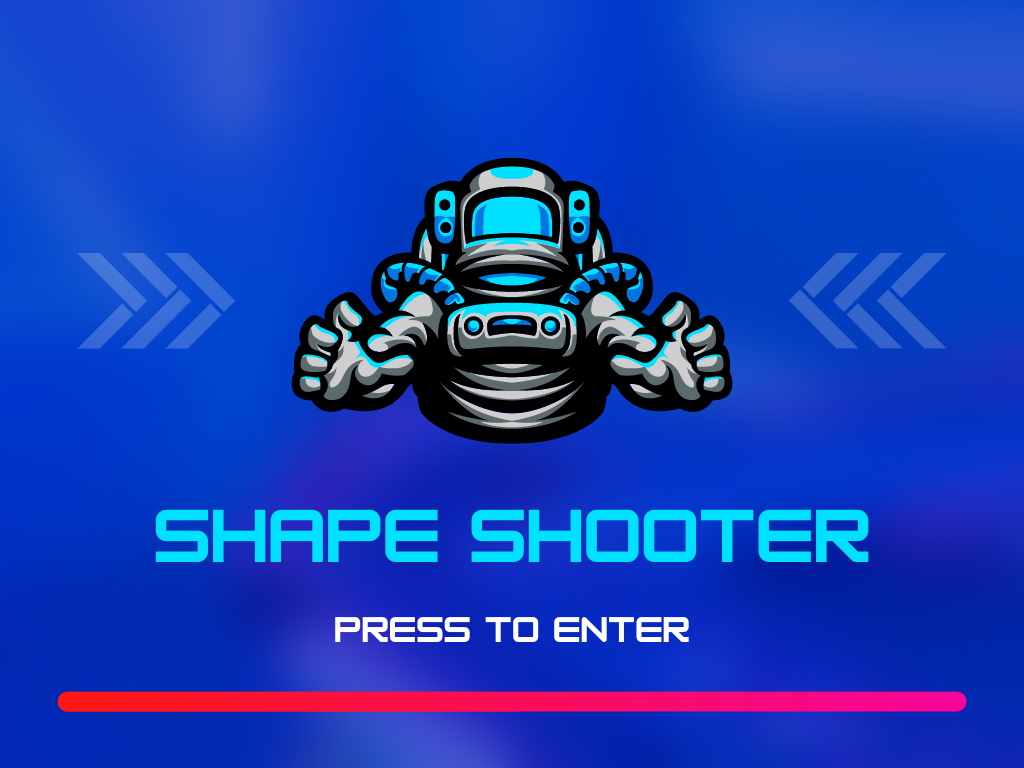
\includegraphics [scale=0.4] {Kravspecifikation/images/spaceshooter.png}
    \caption{Titelskärmen på spelet.}
\end{figure}

\begin{figure}[h!]
    \centering
    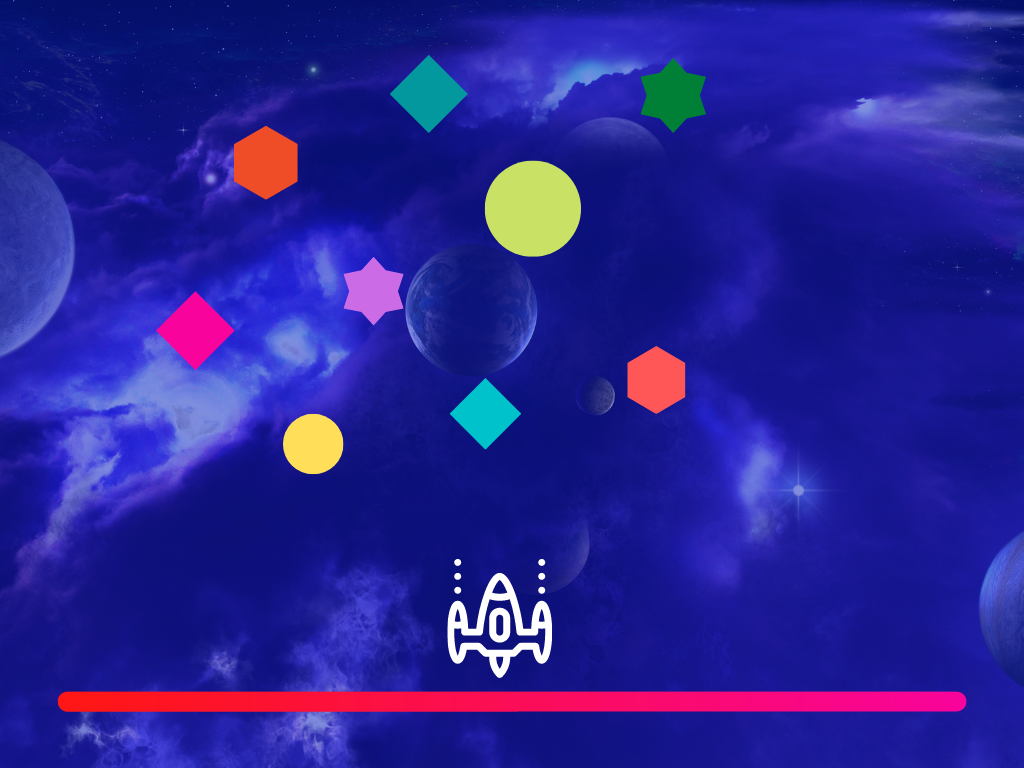
\includegraphics [scale=0.4] {Kravspecifikation/images/game.png}
    \caption{Längst ner i bilden är spelaren som skjuter på fiender och fienderna som flyttar sig mot spelaren.}
\end{figure}

\newpage

\section{Kravformulering}

\subsection{Ska-krav}
1) Spelaren ska kunna röra på sig vänster och höger med hjälp av tangentbordet (← och →).

2) Spelaren ska inte kunna röra sig utanför spelplanens kanter.

3) Spelaren ska kunna skjuta.

4) Om spelaren missar fienden kommer skottet att försvinna.

5) Om fiender blir träffad ska skottet försvinna.

6) Om fienden dör ska både skottet och fienden försvinna från spelplanen.

7) Fiender ska röra sig uppifrån neråt i realtid.

8) När de når spelplanens sida ska de förflyttas neråt.

9) Det ska finnas fiender i olika former.

10) Om en kollision mellan spelare och fiende sker ska den påverka spelarens health-point negativt.

11) Om spelaren lyckas döda alla fiender ska ett segermeddelande visas.

12) En tvådimensionell värld/spelplan ska ritas ut. 

13) Spelet ska kunna läsa filer för banor.

14) Programkoden ska innehålla funktioner för att hjälpa till att lägga till/ändra banor i spelet.

\subsection{Bör-krav}
15) Den ska finnas en timer under spelet.

16) Den ska finnas en health-bar som ändras vid träff eller kollision. 

17) En titelskärm bör finnas (se Figur 1). I den ska man kunna trycka space-knappen för att starta spelet.

18) Spelplanen bör ha en bakgrundsbild (se Figur 2).

19) Spelare och fiender bör ha sprites (se Figur 2).

20) Spelet bör ha points(poäng) när skotten träffar fiender.

21) Fiender bör röra sig snabbare ju mindre fiender som finns kvar i spelplanen.

22) Det bör finnas en paus meny som stoppar spelet (som kallas när man trycker tangentknapp Esc).

23) I paus bör man kunna välja att fortsätta spelet eller avsluta spelet.

\section{Kravuppfyllelse}
För att klara ett funktionellt spel siktas det mot att prioritera på ska-kraven först.

\subsection{\textit{Spelet ska simulera en värld som innehåller olika typer av objekt. Objekten ska ha olika beteenden och röra sig i världen och agera på olika sätt när de möter andra objekt.}}

Världen kommer att bestå av spelarobjektet och fiendeobjekterna. Spelaren kommer att röra sig enligt kommandon (1) och fienderna kommer att röra sig närmare (7) (8). Interaktionerna mellan objekten kommer vara via skjutning (3) (5) och kollisioner (10).

För bör-kraven kommer spelaren få poäng när dennes skott träffar fienden och röra sig snabbare (21).

\subsection{\textit{Det måste finnas minst tre olika typer av objekt och det ska finnas flera instanser av minst två av dessa. T.ex ett spelarobjekt och många instanser av två olika slags fiendeobjekt.}}

Spelarobjektet och flera olika fiendeobjekt (9) kommer att finnas. Instanserna då spelaren och fienderna samspelar kommer vara via skjutning (3) (5) (6) och kollisioner (10).

För bör-kraven kommer fienderna inte kunna skjuta på spelaren (20).

\subsection{\textit{Ett beteende som måste finnas med där figurerna ska röra sig över skärmen. Rörelsen kan följa ett mönster och/eller vara slumpmässig. Minst ett objekt, utöver spelaren ska ha någon typ av rörelse.}}

Spelaren kommer att kunna röra sig vänster och höger (1) och fienderna kommer att röra sig i ett mönster (7) (8).

\subsection{\textit{En figur ska styras av spelaren, antingen med tangentbordet eller med musen. Du kan även göra ett spel där man spelar två stycken genom att dela på tangentbordet (varje spelare använder olika tangenter). Då styr man var sin figur.}}

Spelaren kommer att representeras av en figur. Om bör-kraven uppfylls kommer den att representeras av en sprite (19). Tangentbordet kommer att användas för att förflytta spelaren (1).

\subsection{\textit{Grafiken ska vara tvådimensionell.}}

En tvådimensionell spelplan kommer att ritas ut (12).

\subsection{\textit{Världen (spelplanen) kan antas vara lika stor som fönstret (du kan göra en större spelplan med scrollning, men det blir lite krångligare).}}

Spelplanen kommer vara fixerad (12) och fönsterstorleken kommer därför inte behöva ändringar.

\subsection{\textit{Det ska finnas kollisionshantering, det vill säga, det ska hända olika saker när objekten möter varandra, de ska påverka varandra på något sätt. T.ex kan ett av objekten tas bort, eller så kan objekten förvandlas på något sätt, eller så kan ett nytt objekt skapas. (Ett exempel på att skapa/ta bort objekt är när man i Space Invaders trycker på skjuta-knappen, t.ex en musknapp, då avfyras ett laserskott och skottet blir då en ny figur som skapas och placeras i världen, på en position vid laserkanonens mynning. Skottet rör sig framåt (uppåt) och om det träffar ett fiendeskepp tas både skottet och skeppet bort, om skottet kommer utanför spelplanen, dvs det missar, tas det endast bort.)}}

Kollisioner kommer hanteras av skott (5) (6) och kollision mellan spelare och fiender (10). Om spelaren missar kommer skottet tas bort. Beroende på fienden kommer skottet antingen att ta bort fienden eller kommer skottet bara försvinna och sedan i nästa skott ta bort fienden. Om en kollision mellan spelare och fiende sker kommer spelet att avslutas.

\subsection{\textit{Det ska vara enkelt att lägga till eller ändra banor i spelet. Detta kan exempelvis lösas genom att läsa in banor från en fil (lite som i Sokoban-labben i TDP002), eller genom att ha funktioner i programkoden som bygger upp en datastruktur som definierar en bana.}}

Nya banor kommer att kunna skapas genom att skapa textfiler som spelet sedan kan läsa in (13) (14).

\subsection{\textit{Spelet måste upplevas som ett sammanhängande spel som går att spela!}}

Alla ska-krav kommer att uppfylla detta, särskilt segermeddelandet (11) och game over-meddelandet (10).

\end{document}
